% !TEX encoding = UTF-8 Unicode
% XeLaTeX can use any Mac OS X font. See the setromanfont command below.
% Input to XeLaTeX is full Unicode, so Unicode characters can be typed directly into the source.

% The next lines tell TeXShop to typeset with xelatex, and to open and save the source with Unicode encoding.

%!TEX TS-program = xelatex
%\documentclass[UTF8,a4paper,12pt]{ctexart}%需要UTF8编码

\documentclass[12pt]{article}
\usepackage[bottom=3cm]{geometry}                % See geometry.pdf to learn the layout options. There are lots.
\geometry{letterpaper}       
\usepackage{graphicx}
\usepackage{amssymb}
\usepackage{calc}
\usepackage{hyperref}
\pagestyle{empty}


%CJK Font Setup
\usepackage{fontspec}
\usepackage[PunctStyle=kaiming,AutoFakeBold=false,AutoFakeSlant=false]{xeCJK}
%\setCJKmainfont[BoldFont={Songti SC Bold},ItalicFont={KaiTi}] {SimSun}
%\setCJKsansfont[BoldFont={Heiti SC Medium}]{Heiti SC}
%\setCJKmonofont[BoldFont={Hiragino Sans GB W6}]{Hiragino Sans GB W3}

%English Font Setup
\defaultfontfeatures{Ligatures=TeX}
\setmainfont{Times New Roman}
\setCJKmainfont{SimSun} %中文字体
\setCJKsansfont{SimHei} %中文无衬线字体
\setsansfont[Scale=MatchLowercase]{Arial}
\setmonofont[Scale=MatchLowercase]{Courier New}


\newlength{\Han}
\settowidth{\Han}{汉}
\newcommand{\spreadCJK}[2]{\makebox[#1\Han][c]{#2}}

\begin{document}
\setlength{\headsep}{0cm}

\vspace{\stretch{3}}

\begin{figure}[htbp]
\begin{center}
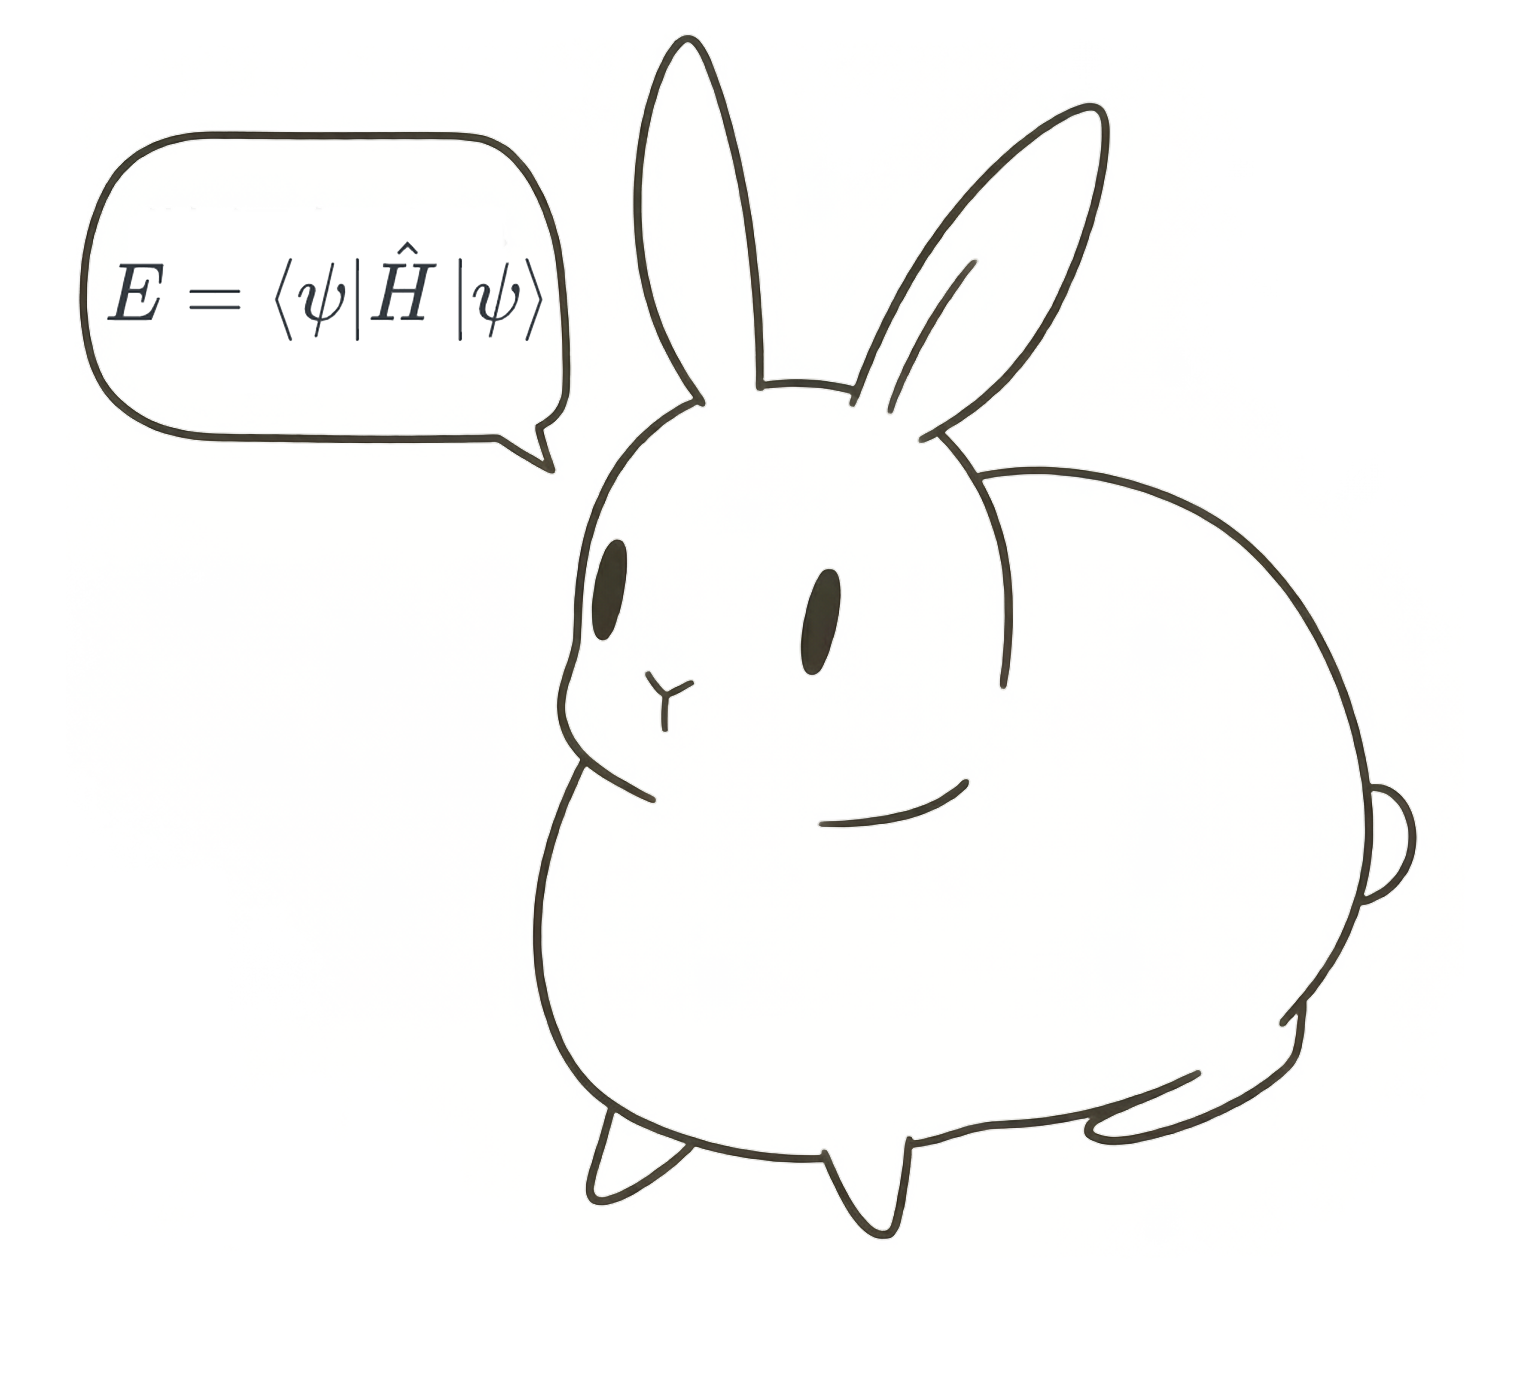
\includegraphics[width=0.7\textwidth]{Speak like Heisenberg.png}
\\
\large{Speak like Heisenberg, Think like Schrödinger, and Work like Dirac.}
\end{center}
\end{figure}

\vspace{\stretch{0.5}}
\begin{center}
\vspace{\stretch{1.5}}
{\LARGE \textsf{从公理、模型到计算实验的量子化学入门}\par}
\vspace{\stretch{0.5}}
{\LARGE \textrm{A Journey to Quantum Chemistry}\par}
\vspace{\stretch{0.5}}
\Large Volume I \\
\vspace{\stretch{2}}
\today

\end{center}

\end{document}  